\documentclass{ctexart}
\usepackage{geometry}
\usepackage{amsmath}
\usepackage{listings}
\usepackage[dvipsnames]{xcolor}
\usepackage{cite}
\usepackage{diagbox}
\usepackage{fancyhdr} % 加载fancyhdr宏包,用于设置页眉和页脚
\pagestyle{fancy} % 设置页面样式
\fancyhf{} % 清除默认的页眉和页脚的内容
\fancyfoot[C]{\thepage} 
\renewcommand{\headrulewidth}{0pt} % 将页眉的横线宽度设置为0pt
% \usepackage[left=1.5cm,right=1.5cm,top=1.5cm,bottom=1.5cm]{geometry}
\usepackage[left=0.1cm,right=0.1cm,top=0.1cm,bottom=0.1cm]{geometry}
\usepackage{graphics}
\usepackage{longtable}
\usepackage{tabularx}
\usepackage{float}
\usepackage{amsmath}%引用宏包要放在documentclass后面,否则报错
\usepackage{hyperref}
\usepackage{bm}
\usepackage{amssymb}
\usepackage{esint}
\usepackage{booktabs}
%\usepackage{subfiles}%用于分章节管理引用,使各章节引用来源于各自的文件,编号相互独立
\usepackage{amsthm}
\title{数字电路实验3\quad 实验报告}
\author{Leo}
\date{\today}

\begin{document}
\maketitle
\section{实验内容}
用74151实现密码锁。具体要求为:
\begin{enumerate}
    \item 密码为四位二进制数
    \item 密码在设计时确定,不可更改
    \item 当用户输入正确的密码且确认开启密码锁时,才会开启密码锁(用亮绿灯来表示).其余情况均亮红灯
\end{enumerate}

\section{实验器材}
Pocketlab、电脑、导线若干、剥线钳、镊子、限流电阻2个、红色和绿色LED灯各一个、74151芯片一个。芯片的引脚图如图\ref{fig:74151引脚图}所示
\begin{figure}[H]
    \centering
    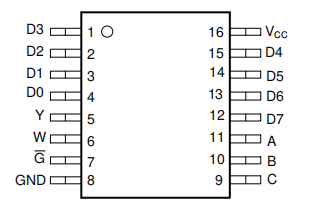
\includegraphics[width=0.4\linewidth]{74151.png}
    \caption{74151引脚图}
    \label{fig:74151引脚图}
\end{figure}
\section{实验原理}
% 题目要求识别2421BCD码中的伪码,若设输入变量为A,B,C,D,输出为F,并规定伪码输出为1,有效码输出为0,则可以列出如下真值表
题目要求识别出用户输入的密码是否为预先设定密码值。在这里我们不妨规定,有效的密码输出P为高电平,其余输出为低电平;开锁信号Q当确认开锁时为低电平,不开锁时为高电平。预设密码值定为1011.于是我们可以列出F的真值表。
\begin{longtable}{|p{2cm}<{\centering}| p{2cm}<{\centering} |p{2cm}<{\centering}| p{2cm}<{\centering} |p{2cm}<{\centering}|  p{2cm}<{\centering}|}%手动调间距
\caption{真值表}
\hline
  A & B & C & D & Q & F \\
\hline
  x & x& x &x &1 & 0\\
\hline
  0 & 0 & 0 & 0 & 0 & 0 \\
\hline
  0 & 0 & 0 & 1 & 0 & 0 \\
\hline
  0 & 0 & 1 & 0 & 0 & 0 \\
\hline
  0 & 0 & 1 & 1 & 0 & 0 \\
\hline
  0 & 1 & 0 & 0 & 0 & 0 \\
\hline
  1 & 0 & 1 & 1 & 0 & 1 \\
\hline
  1 & 1 & 0 & 0 & 0 & 0 \\
\hline
  1 & 1 & 0 & 1 & 0 & 0 \\
\hline
  1 & 1 & 1 & 0 & 0 & 0 \\
\hline
  1 & 1 & 1 & 1 & 0 & 0 \\
\hline
  0 & 1 & 0 & 1 & 0 & 0 \\
\hline
  0 & 1 & 1 & 0 & 0 & 0 \\
\hline
  0 & 1 & 1 & 1 & 0 & 0 \\
\hline
  1 & 0 & 0 & 0 & 0 & 0 \\
\hline
  1 & 0 & 0 & 1 & 0 & 0 \\
\hline
  1 & 0 & 1 & 0 & 0 & 0 \\
\hline
\end{longtable}
对应真值表可以做出当开锁信号为有效时的卡诺图
\begin{table}[H]
    \centering
    \caption{卡诺图}
    \begin{tabular}{|c|c|c|c|c|}
\hline
\diagbox{AB}{CD} & 00 & 01 & 11 & 10 \\
\hline
00 & 0 & 0 & 0 & 0  \\
\hline
01 & 0 & 0 & 0 & 0  \\
\hline
11 & 0 & 0 & 0 & 0  \\
\hline
10 & 0 & 0 & 1 & 0  \\
\hline
\end{tabular}
    \label{tab:卡诺图}
\end{table}
考虑到74151只有三个输入变量的端口,若只使用一片74151,则需要将一位变量降维,这里我们选择将D降维。降维后的卡诺图为
\begin{table}[H]
    \centering
    \caption{降维后的卡诺图}
    \begin{tabular}{|c|c|c|}
\hline
\diagbox{AB}{C} & 0 &1 \\
\hline
00 & 0 & 0   \\
\hline
01 & 0 & 0   \\
\hline
11 & 0 & 0   \\
\hline
10 & 0 & D \\
\hline
\end{tabular}
    \label{tab:降维后的卡诺图}
\end{table}
% 写出逻辑函数的表达式
%连等式的写法
对应的函数表达式为
\begin{equation}
F=Q' \cdot (AB'CD)
\end{equation}
\section{电路设计与实现}
\subsection{电路仿真图}
在Multisim中连接好电路仿真图
\begin{figure}[H]
    \centering
    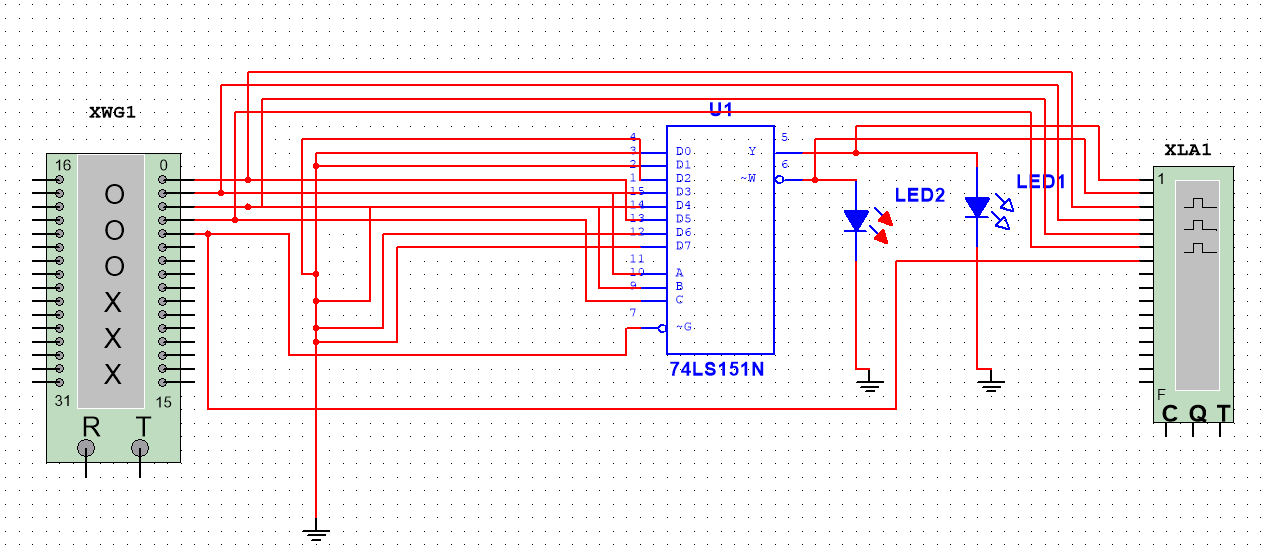
\includegraphics[width=0.6\linewidth]{multisim仿真图.png}
    \caption{Multisim仿真电路图}
    \label{fig:Multisim仿真电路图}
\end{figure}
在本次实验中,如果算上开锁信号Q,则一共有32种输入组合,不便于用开关控制输入与输出。这里采用字发生器和逻辑分析仪进行仿真。如下是逻辑分析仪显示的波形图
\begin{figure}[H]
    \centering
    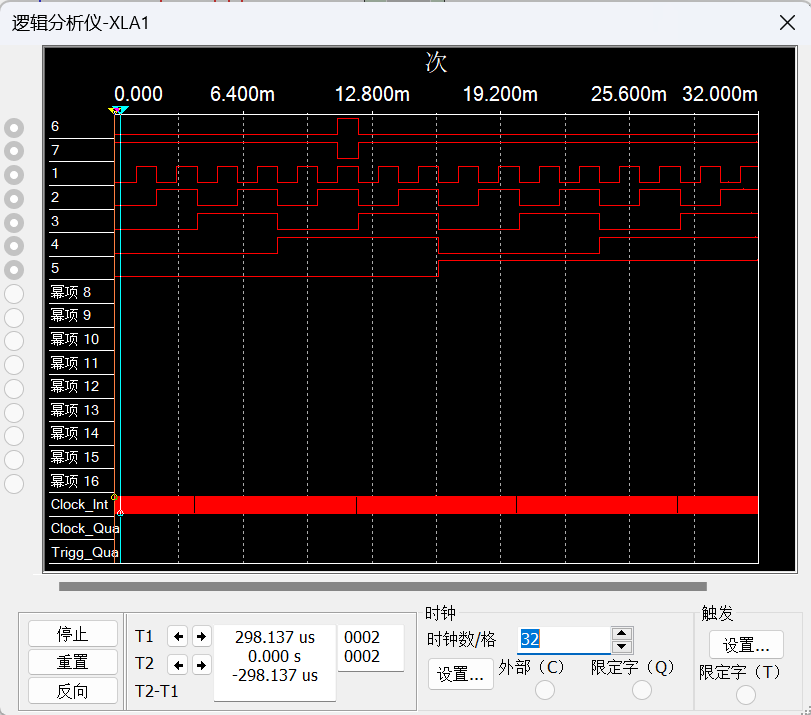
\includegraphics[width=0.6\linewidth]{逻辑分析仪.png}
    \caption{逻辑分析仪波形图}
    \label{fig:逻辑分析仪波形图}
\end{figure}
可以看到,输出的信号满足设计要求,即仅在开锁信号有效且密码正确的情况下,锁被打开。
\subsection{电路实物图}
按电路仿真图搭好实物电路图
\begin{figure}[H]
    \centering
    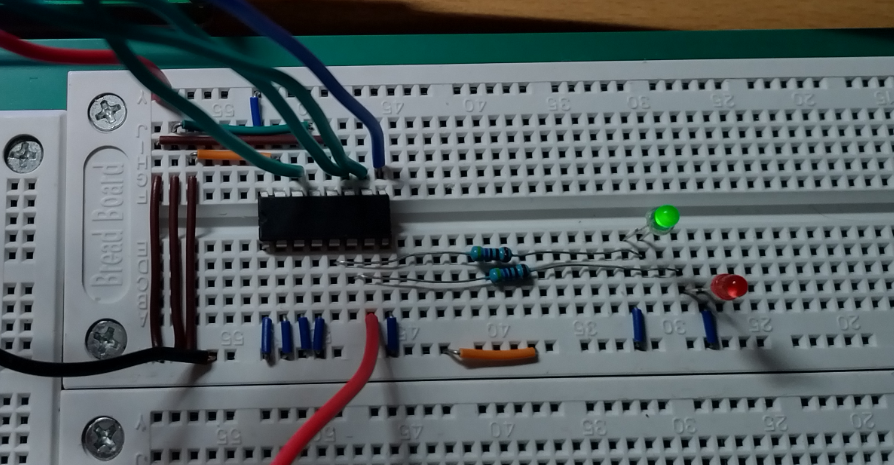
\includegraphics[width=0.6\linewidth]{实际电路图.png}
    \caption{实物电路图}
    \label{fig:实物电路图}
\end{figure}
\section{功能测试}
运行PocketLab,逐一测试输入。如图是Pocketlab逻辑分析仪的部分实验截图
\begin{figure}[H]
    \centering
    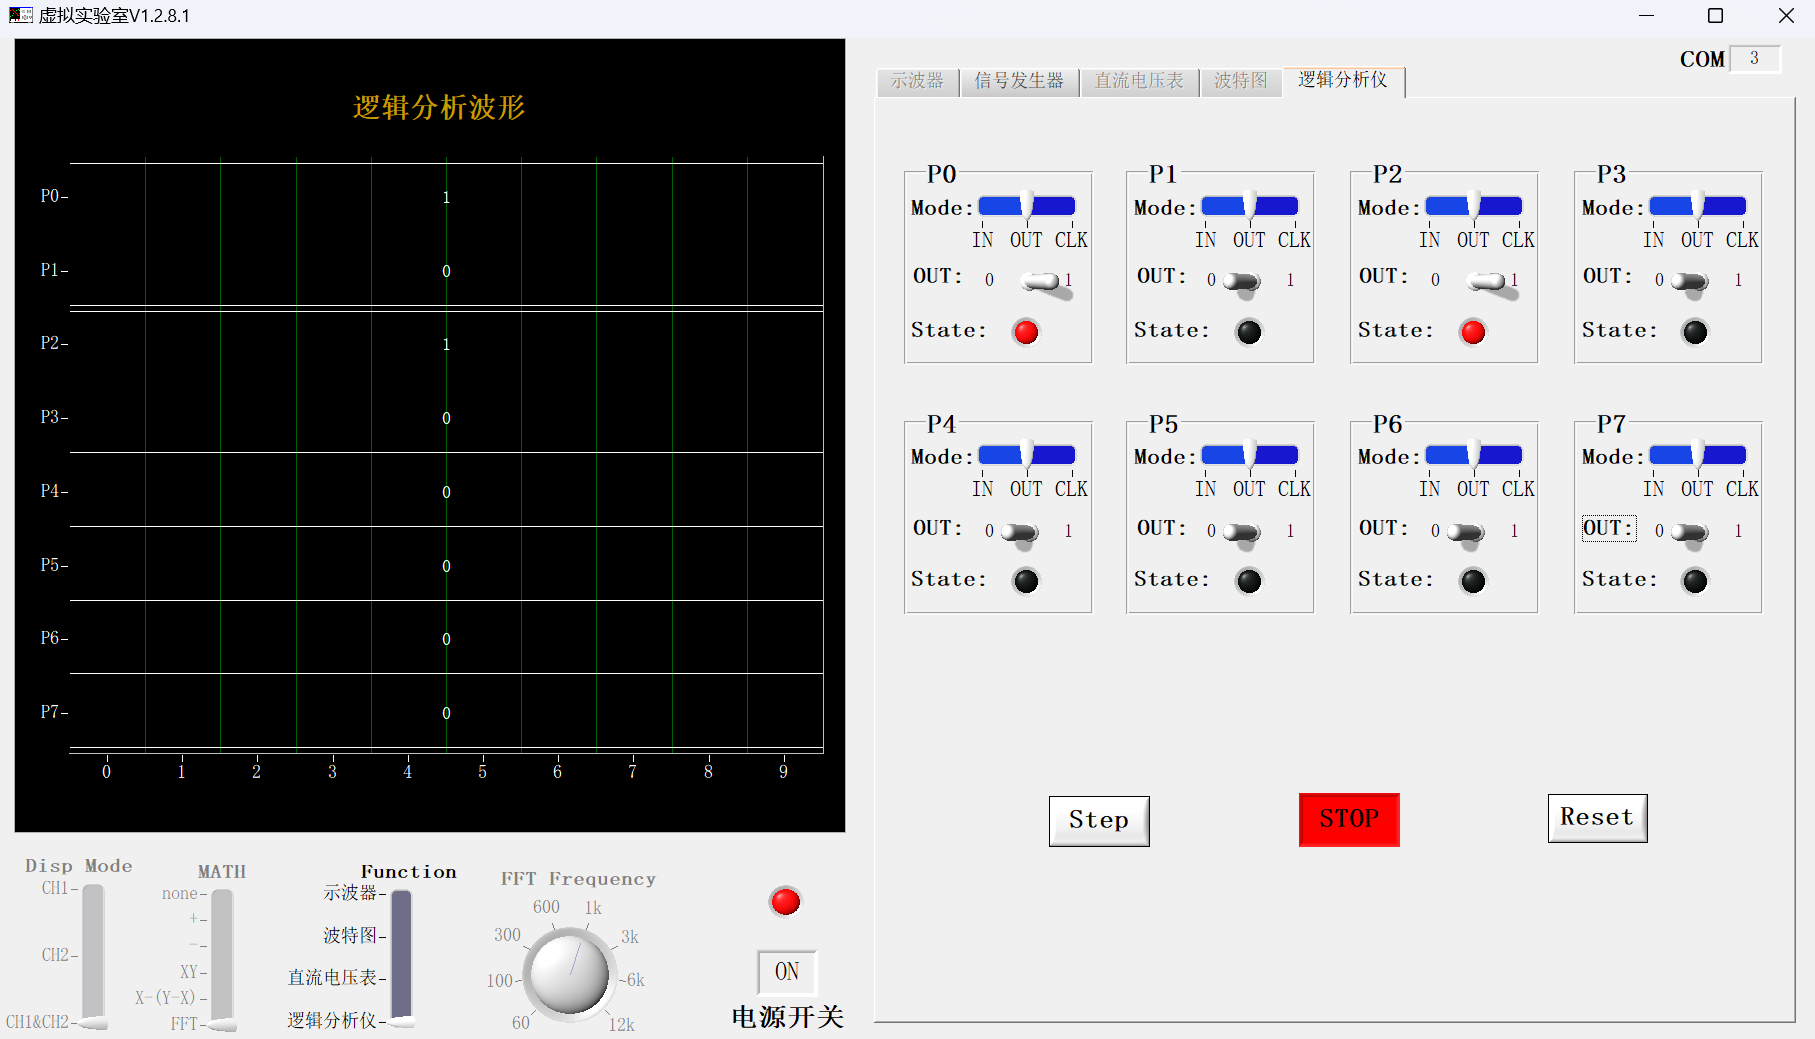
\includegraphics[width=0.6\linewidth]{密码不正确但开锁.png}
    \caption{密码错误,开锁信号有效,显示为红灯}
    \label{fig:密码错误,开锁信号有效,显示为红灯}
\end{figure}
\begin{figure}[H]
    \centering
    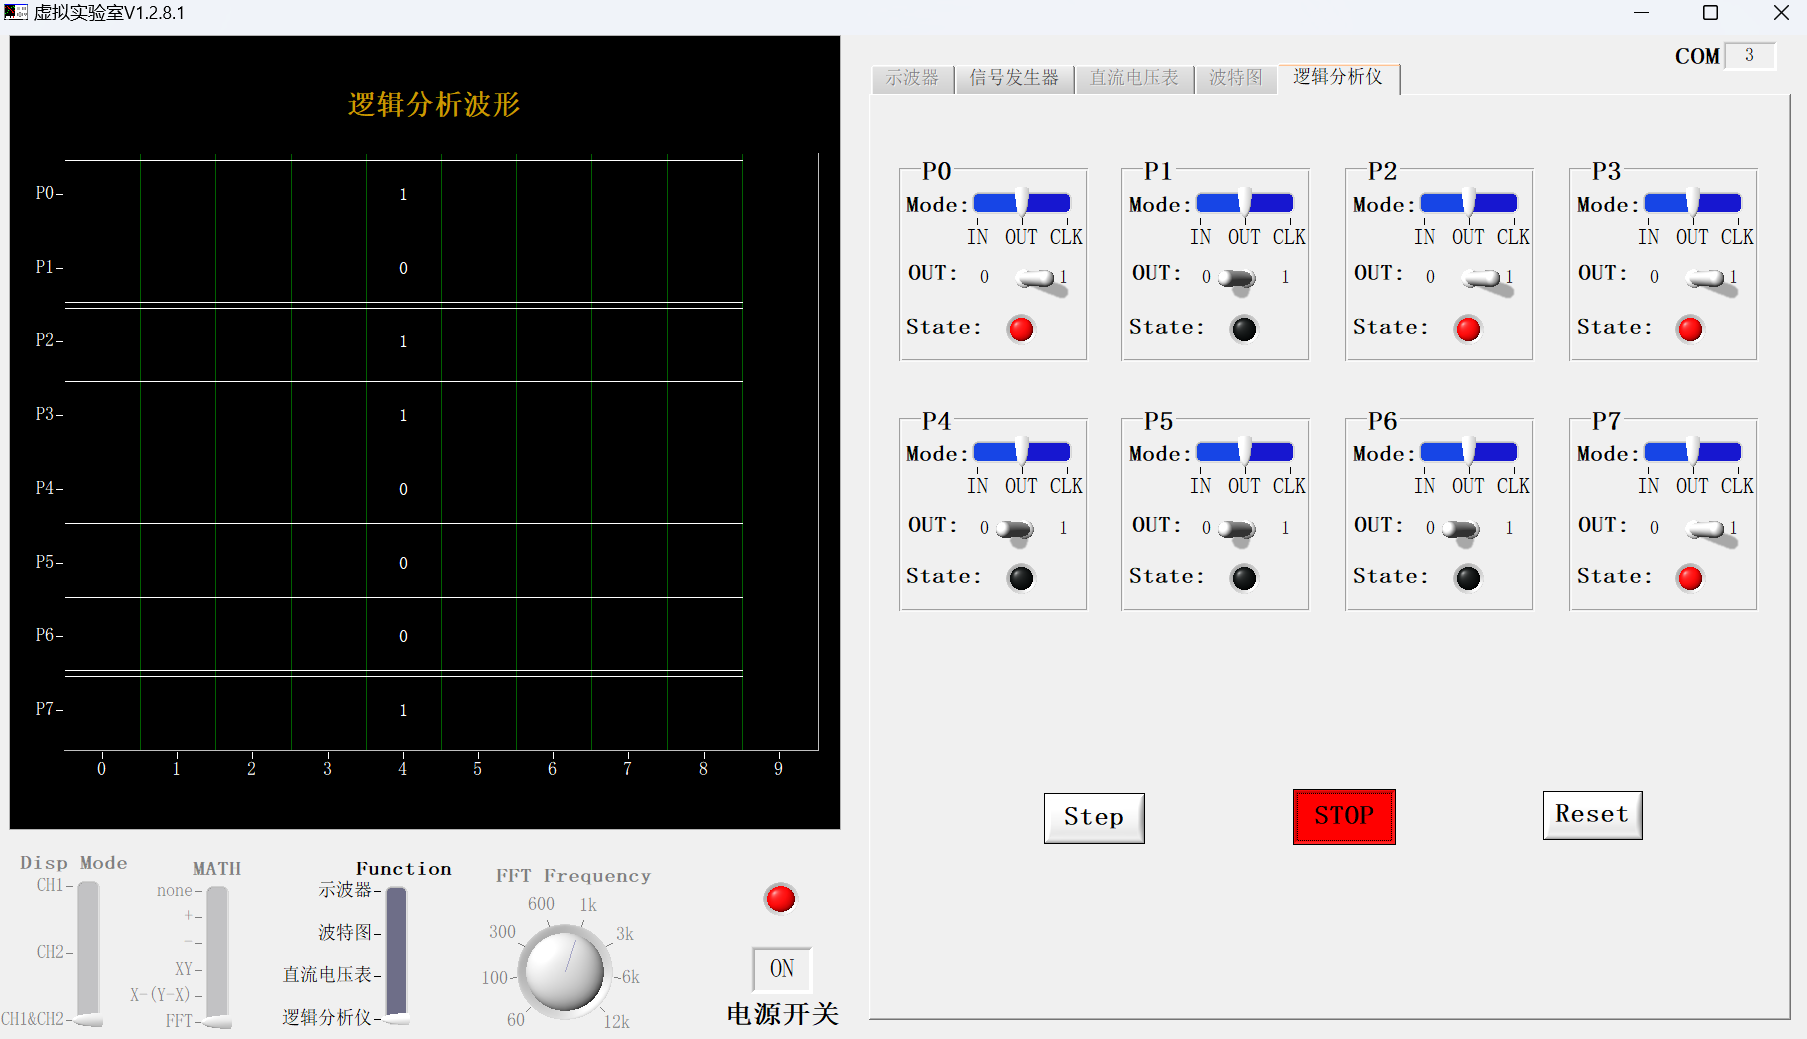
\includegraphics[width=0.6\linewidth]{密码正确但不开锁.png}
    \caption{密码正确,开锁信号无效,显示为红灯}
    \label{fig:密码正确,开锁信号无效,显示为红灯}
\end{figure}
\begin{figure}[H]
    \centering
    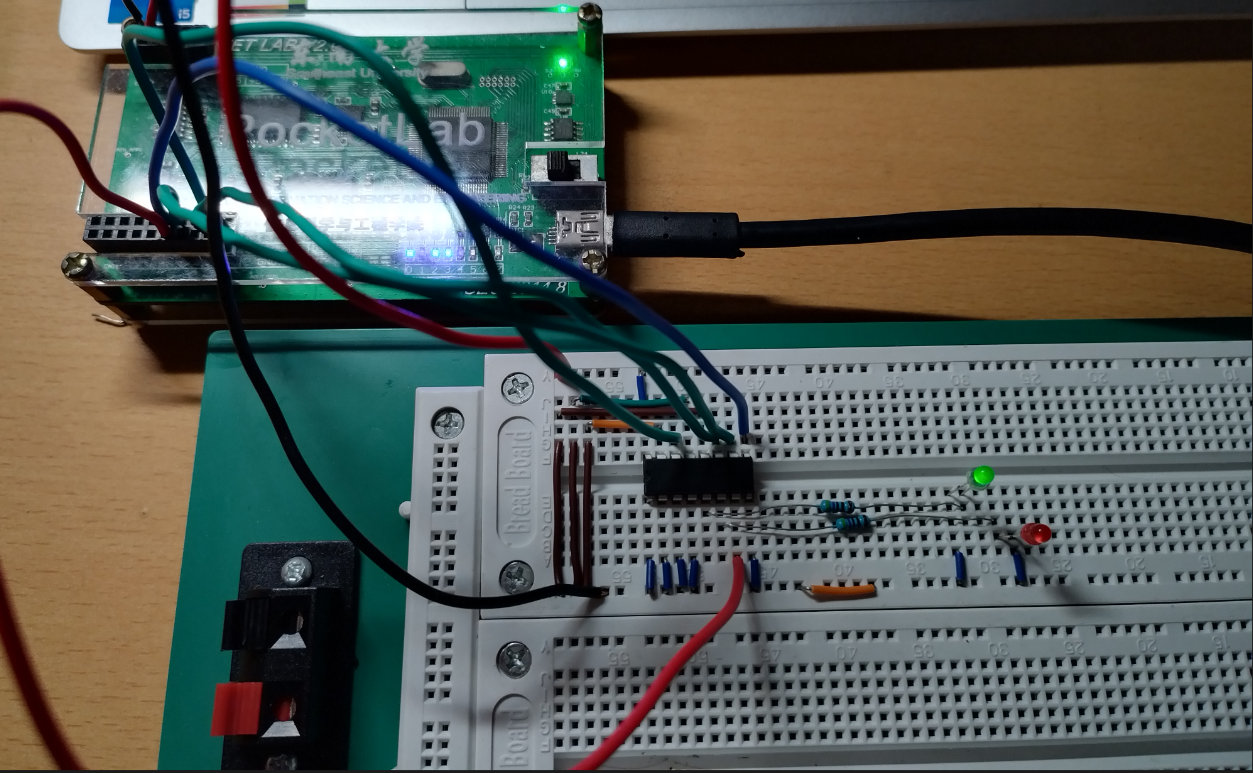
\includegraphics[width=0.6\linewidth]{image.png}
    \caption{密码正确,开锁信号有效,显示为绿灯}
    \label{fig:密码正确,开锁信号有效,显示为绿灯}
\end{figure}
下面是实物电路图的照片,分别对应开锁成功与开锁失败时恶的亮灯情况
\begin{figure}[H]
    \centering
    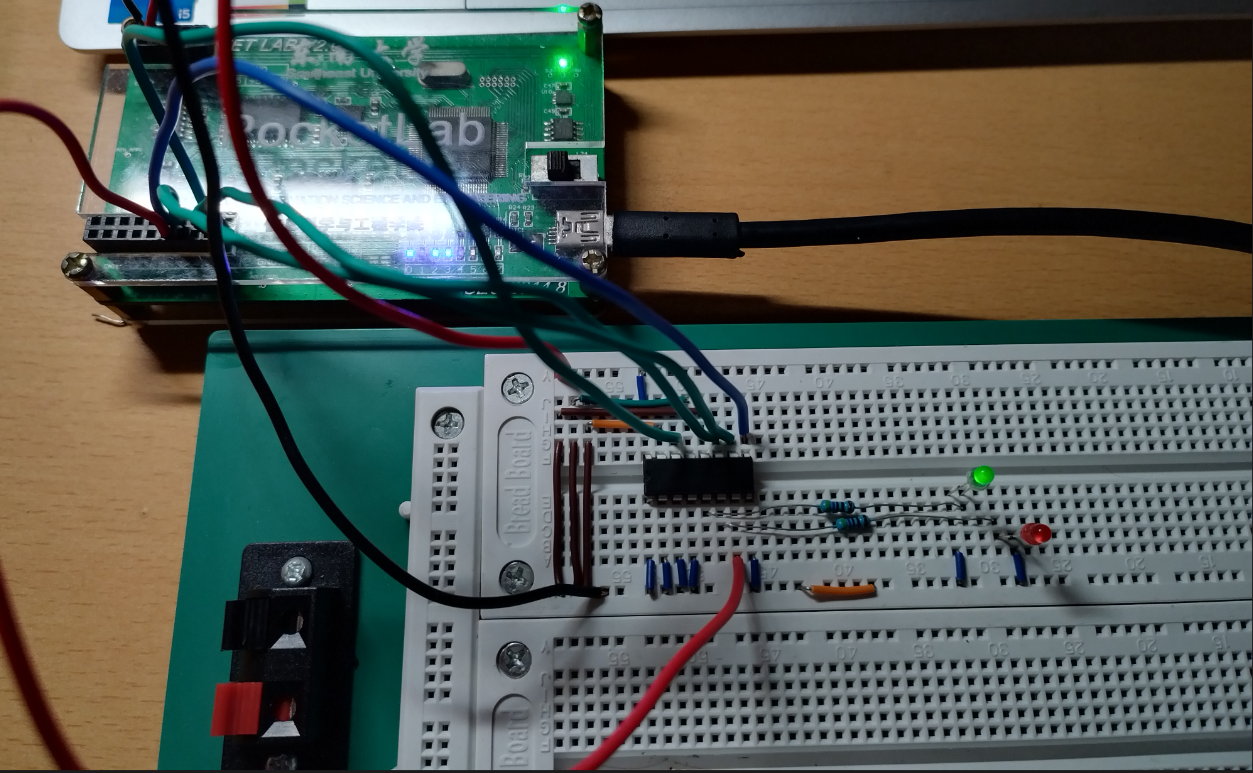
\includegraphics[width=0.6\linewidth]{实物1.png}
    \caption{开锁成功}
    \label{fig:开锁成功}
\end{figure}
\begin{figure}[H]
    \centering
    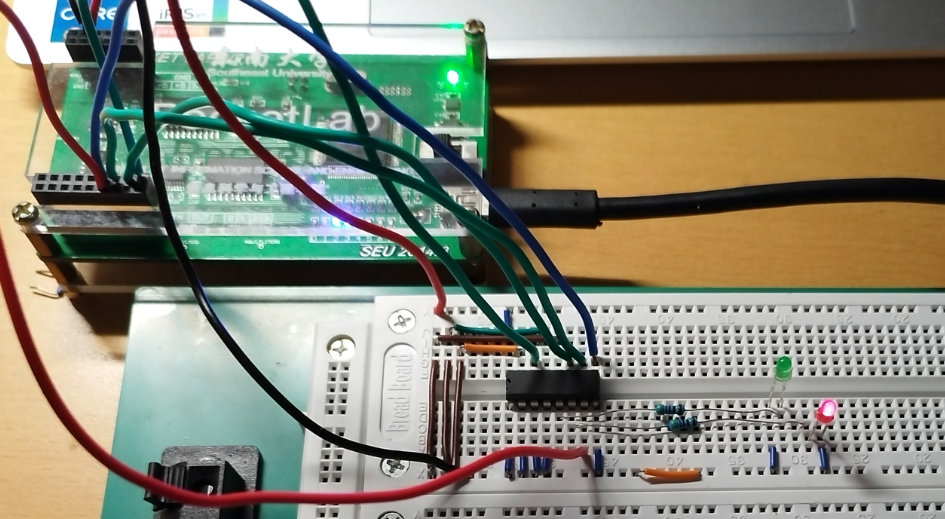
\includegraphics[width=0.6\linewidth]{实物2.png}
    \caption{开锁失败}
    \label{fig:开锁失败}
\end{figure}
\section{实验总结与反思}
本次实验较为简单,从仿真到搭建实际电路都更加熟练。特别是在Multisim仿真时学会使用字发生器和逻辑分析仪,给电路输出信号的分析带来的极大便利。

本次实验的不足之处在于:第一版设计没有实现最小化。第一次设计电路时,没有想到可以将开锁信号放在使能端,而是将74151的输出信号与开锁信号放在一起做与非运算再取非,思路比较简单但是不够高效。
\end{document}